% The primes and residue fields in the quadratic reciprocity proof:
% 𝔓 in ℤ[ζ_q] above 𝔭 in 𝒪_K above (p) in ℤ.
% Source: book/tex/alg-NT/frobenius.tex (§ Application: Quadratic
% reciprocity, Step 2) — tikzcd.
\documentclass[border=2mm]{standalone}
\usepackage{tikz}
\usetikzlibrary{arrows.meta}
\usepackage{amssymb}
\usepackage{amsmath}
\begin{document}
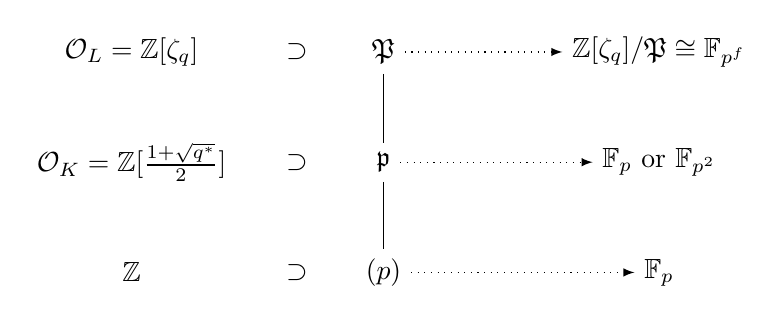
\begin{tikzpicture}[>=latex]
  \node (OL) at (0,2.8)   {$\mathcal{O}_L = \mathbb{Z}[\zeta_q]$};
  \node (OK) at (0,1.4)   {$\mathcal{O}_K = \mathbb{Z}[\frac{1+\sqrt{q^\ast}}{2}]$};
  \node (Z)  at (0,0)     {$\mathbb{Z}$};
  \node (s1) at (2.1,2.8) {$\supset$};
  \node (s2) at (2.1,1.4) {$\supset$};
  \node (s3) at (2.1,0)   {$\supset$};
  \node (PP) at (3.2,2.8) {$\mathfrak{P}$};
  \node (pp) at (3.2,1.4) {$\mathfrak{p}$};
  \node (p)  at (3.2,0)   {$(p)$};
  \node (F1) at (6.7,2.8) {$\mathbb{Z}[\zeta_q]/\mathfrak{P} \cong \mathbb{F}_{p^f}$};
  \node (F2) at (6.7,1.4) {$\mathbb{F}_p$ or $\mathbb{F}_{p^2}$};
  \node (F3) at (6.7,0)   {$\mathbb{F}_p$};
  \draw (PP) -- (pp) -- (p);
  \draw[dotted, ->] (PP) -- (F1);
  \draw[dotted, ->] (pp) -- (F2);
  \draw[dotted, ->] (p) -- (F3);
\end{tikzpicture}
\end{document}
